% Figura das matrizes de correlacao (Secao III do artigo ICIT 2027).
% PDFs gerados por: plot_matriz_correlacao_final(false, true, true)
% Subir no Overleaf: matriz_2700rpm.pdf, matriz_3000rpm.pdf, matriz_3500rpm.pdf
% Preambulo: \usepackage[caption=false,font=footnotesize]{subfig} e \usepackage{siunitx}
% Legenda ainda nao confirmada pelo usuario.

\begin{figure*}[!t]
\centering
\subfloat[]{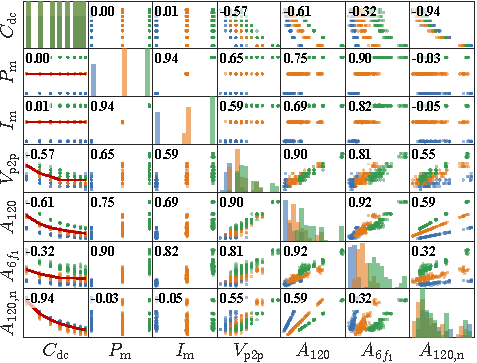
\includegraphics[width=0.32\textwidth]{matriz_2700rpm.pdf}\label{fig:matriz_2700}}\hfil
\subfloat[]{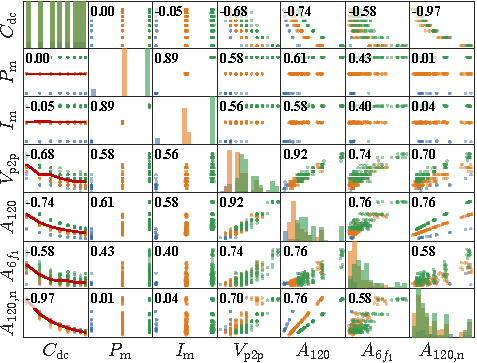
\includegraphics[width=0.32\textwidth]{matriz_3000rpm.pdf}\label{fig:matriz_3000}}\hfil
\subfloat[]{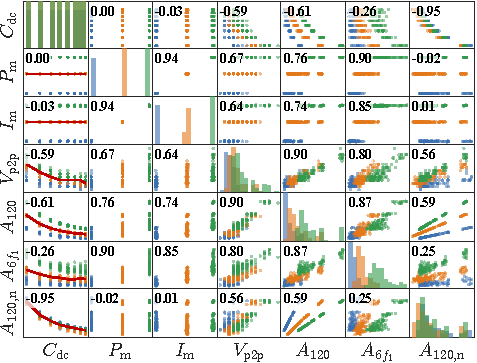
\includegraphics[width=0.32\textwidth]{matriz_3500rpm.pdf}\label{fig:matriz_3500}}
\caption{Spearman correlation matrices of the dc-link capacitance and the extracted features at (a) \SI{2700}{rpm}, (b) \SI{3000}{rpm}, and (c) \SI{3500}{rpm}, with loads of \SI{80}{\watt} (blue), \SI{150}{\watt} (orange), and \SI{210}{\watt} (green). $C$: dc-link capacitance; $P$: load power; $I_m$: motor rms current; $V_{p2p}$: dc-link peak-to-peak voltage; $A_{120}$: amplitude of the \SI{120}{\hertz} dc-link ripple component; $A_{6f_1}$: amplitude of the dc-link component at six times the motor electrical frequency; $A_{120,n} = A_{120}/(V_m I_m)$. The values in each plot are the Spearman coefficients, and the red lines show the median of each feature for each capacitance level.}
\label{fig:matrizes}
\end{figure*}
